\section{Sparse matrix multiplication}
Sparse matrix multiplication on graphs leads to many random memory
accesses and its performance is usually limited by random memory performance
of DRAM. To scale sparse matrix multiplication to a sparse graph with billions
of vertices, we perform this operation in semi-external memory (SEM). That is,
we keep the vector or the dense matrix in memory and the sparse matrix on SSDs.
This strategy enables nearly in-memory performance while achieving
the scalability in proportion to the ratio of non-zero entries to rows or columns
in the sparse matrix.

\subsection{The sparse matrix format}
The state-of-art numeric libraries store a sparse matrix in compressed row storage
(CSR) or compressed column storage (CSC) format. However, these formats incur
many CPU cache misses in sparse matrix multiplication on many real-world graphs
due to their nearly random vertex connection. They also require a relatively
large storage size. For a graph with billions of edges, we have to use eight
bytes to store the row and column indices. For semi-external memory sparse
matrix multiplication, SSDs may become the bottleneck if a sparse matrix has
a large storage size.
Therefore, we need to use an alternative format for sparse matrices to increase
CPU cache hits and reduce the amount of data read from SSDs.

\begin{figure}
\centering
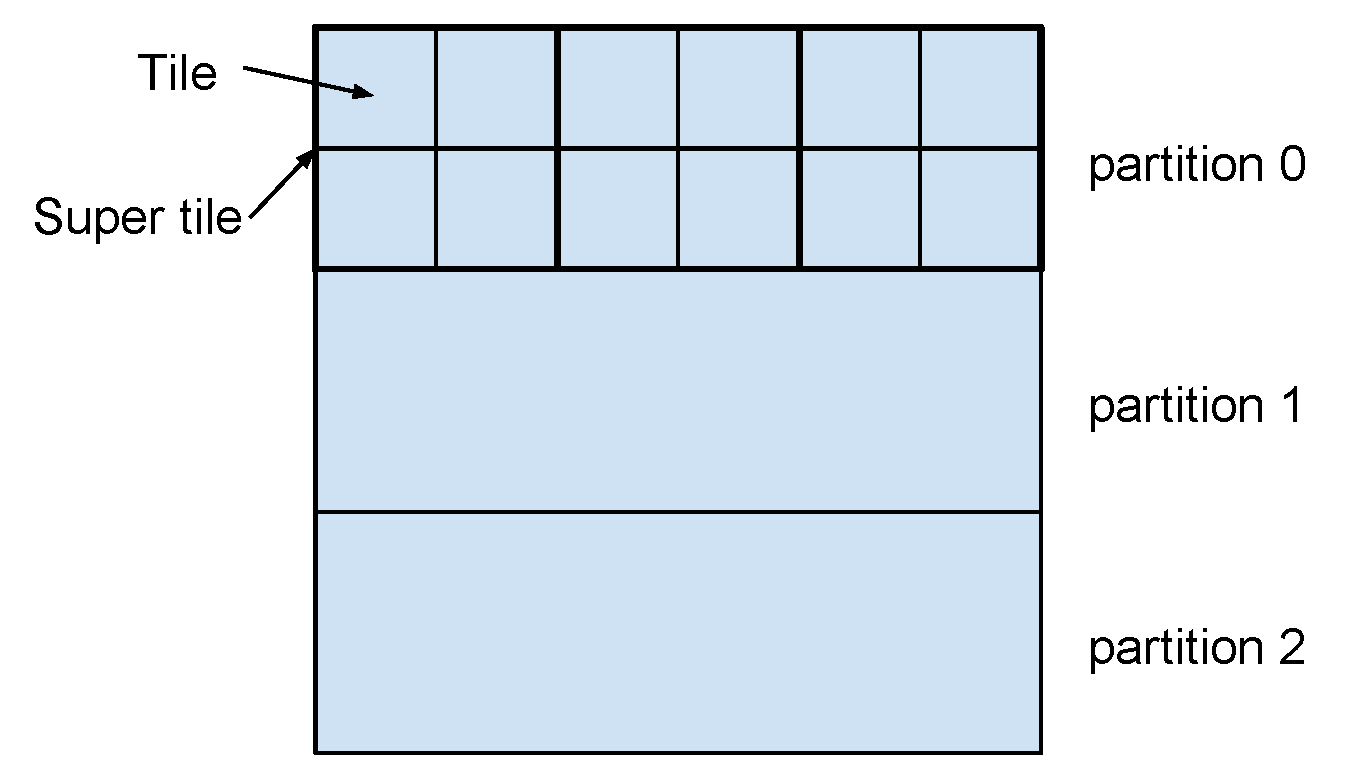
\includegraphics[scale=0.3]{./sparse_mat.pdf}
\caption{The format of a sparse matrix.}
\label{sparse_mat}
\end{figure}

To increase CPU cache hits, we deploy cache blocking \cite{Im04} and store
non-zero entries of a sparse matrix in tiles (Figure \ref{sparse_mat}).
When a tile is small, the rows from the input and output dense matrices
involved in the multiplication with the tile are always kept in the CPU cache
during the computation. The optimal tile size should fill the CPU cache
with the rows of the dense matrices involved in the multiplication with
the tile and is affected by the number of columns of the dense matrices,
which is chosen by users. Instead of generating a sparse matrix with
different tile sizes optimized for different numbers of columns in the dense
matrices, we use a relatively small tile size and rely on the runtime system
to optimize for different numbers of columns (in section \ref{sec:cpu}).
In the semi-external memory, we expect that the dense matrices do not
have more than eight columns in sparse matrix multiplication. Therefore, we
use the tile size of $16K \times 16K$ by default to balance the matrix storage
size and the adaptibility to different numbers of columns.

\begin{figure}
\centering
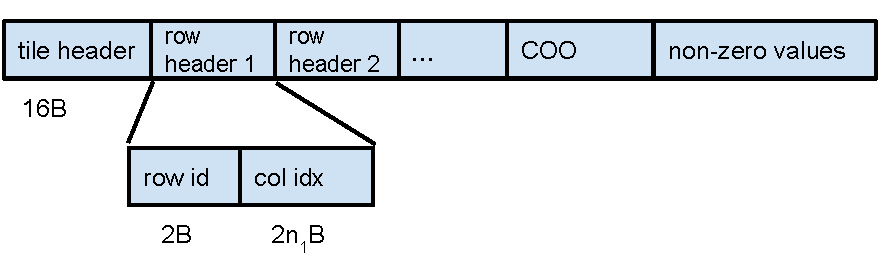
\includegraphics[scale=0.5]{./tile_format.pdf}
\caption{The storage format of a tile in a sparse matrix.}
\label{tile_format}
\end{figure}

To reduce the overall storage size of a sparse matrix, we use a compact format
to store non-zero entries in a tile. In very sparse matrices such as
many real-world graphs, many rows in a tile do not have any non-zero entries.
The CSR (CSC) format requires an entry for each row (column) in the row
(column) index. Therefore, the CSR or CSC format wastes space when storing elements
in a tile. Instead, we only keep data for rows with non-zero entries in a tile
shown in Figure \ref{tile_format} and refer to this format as SCSR (Super
Compressed Row Storage). This format maintains a row header for each non-empty
row. A row header has an identifier to indicate the row number, followed by
column indices. 
The most significant bit of the identifier is always set to 1, while the most
significant bit of a column index entry is always set to 0. As such, we can easily
distinguish a row identifier from a column index entry and determine the end
of a row. Thanks to the small size of a tile, we use two bytes to further store a row
number and a column index entry to reduce the storage size. Since the most
significant bit is used to indicate the beginning of a row, this format allows
a maximum tile size of $32K \times 32K$.

For many real-world graphs, many rows in a tile have only one non-zero entry,
thanks to the sparsity of the graphs and nearly random vertex connection.
Iterating over single-entry rows requires to test the end of a row for every
non-zero entry, resulting in many extra conditional jump CPU instructions
in sparse matrix multiplication.
In contrast, the coordinate format (COO) is more suitable for storing these
single-entry rows. It does not increase the storage size but significantly
reduces the number of conditional jump instructions when we iterate
them. As a result, we hybrid SCSR and COO to store non-zero entries in a tile
with COO stored behind the row headers of SCSR. All non-zero entries are
stored together at the end of a tile.

We organize tiles in a sparse matrix in tile rows and maintain a matrix index
for them. Each entry of the index stores the location of a tile row on SSDs
to facilitate random access
to tile rows. This is useful for parallelizing sparse matrix multiplication.
Because a tile contains thousands of rows, the matrix index requires a very
small storage size even for a billion-node graph. We keep the entire index
in memory during sparse matrix multiplication.

\subsection{The dense matrices}
Dense matrices in sparse matrix multiplication are tall-and-skinny matrices
with millions or even billions of rows but only a small number of columns.
The number of rows in a dense matrix is determined by the number of rows or
columns in a sparse matrix and the number of columns is determined by applications.
We keep the input dense matrix in memory, so its size governs memory consumption
of sparse matrix multiplication. Given the limited amount of RAM in a machine,
the number of columns in a dense matrix has to be small.

For a non-uniform memory architecture (NUMA), we partition the input dense matrix
horizontally and store partitions evenly across NUMA nodes to fully utilize
the bandwidth of memory and inter-processor links in sparse matrix
multiplication. The NUMA architecture is prevalent in today's multi-processor
servers, where each processor connects to its own memory banks. As shown in
Figure \ref{dense_mat} (a), we assign multiple
contiguous rows in a row interval to a partition, which is assigned to a NUMA
node. A row interval always has $2^i$ rows for efficiently locating a row
with bit operations. The row interval size is multiple of the tile size of
a sparse matrix so that multiplication on a tile only needs to access rows
from a single row interval. The elements in the input dense matrix are stored
in row-major order to increase data locality in SpMM.

\begin{figure}
\centering
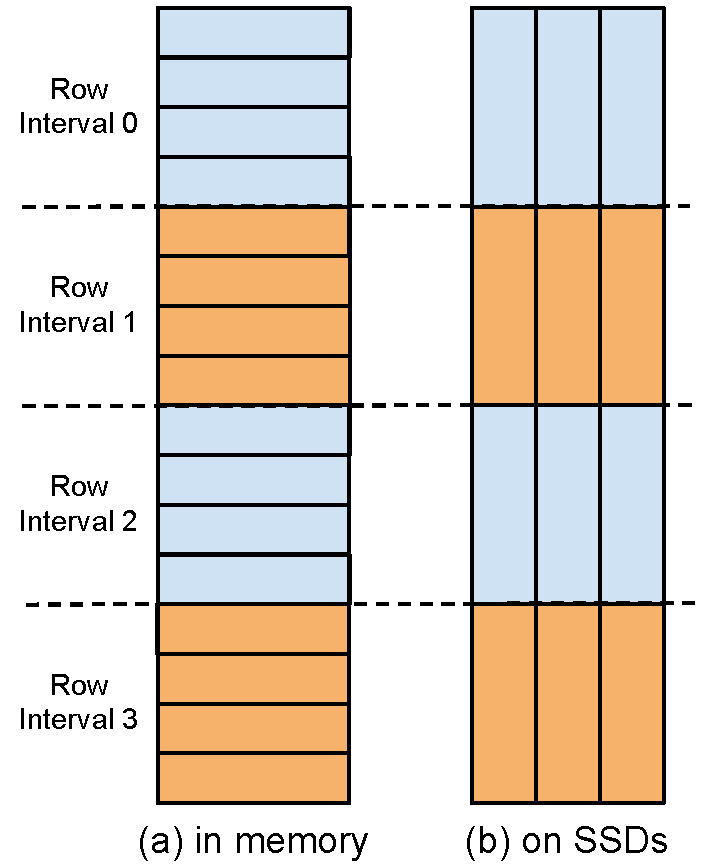
\includegraphics[scale=0.4]{./dense_matrix.pdf}
\caption{The data layout of tall-and-skinny (TAS) dense matrices. A TAS
dense matrix is partitioned horizontally into many row intervals.
(a) For an in-memory matrix, row intervals are stored across NUMA nodes and
elements are stored in row-major order; (b) for an SSD-based matrix, elements
inside a row interval are stored in column-major order.}
\label{dense_mat}
\end{figure}

\subsection{Semi-external memory}
With semi-external memory, we keep the sparse matrix on SSDs and keep the dense
matrix in memory for sparse matrix multiplication. For minimum memory
consumption, we only need to keep the input dense matrix in memory and
stream the output matrix to SSDs during the computation if necessary.
During the computation, we stream data in the sparse matrix from SSDs,
which maximizes I/O throughput of the SSDs.

There are three options of keeping the output dense matrix of sparse matrix
multiplication. In some applications such as PageRank and many other graph
algorithms, dense matrices have only a few columns, so we can keep the output
dense matrix in memory for most of the machines. If a machine has insufficient
memory to keep the output dense matrix, we have to write the output dense matrix
back to SSDs. In this case, we stream the output dense matrix to SSDs when data
is generated. Another option is to stream the data to the subsequent operations
if a machine does not have sufficient memory. \dz{I need to implement this.}
As such, we significantly reduce I/O.

In some applications such as non-negative matrix factorization shown in Section
\ref{sec:app}, even the input dense matrix cannot fit in memory. In this case,
we partition the input dense matrix vertically so
that each partition has complete columns of the original dense matrix and can
fit in memory. We organize each partition in the row-major order to increase
data locality. For each partition, we perform sparse matrix multiplication
in semi-external memory as before and stream the output matrix to SSDs.
This approach requires $\lceil \frac{D}{M} \rceil$ passes over the sparse matrix,
where $D$ is the storage size of the input dense matrix and $M$ is the memory
size.

\subsection{Parallelization}
When parallelizing sparse matrix multiplication, we need to take into account
semi-external memory as well as the power-law distribution of non-zero entries
in each row of the sparse matrix.

We partition a sparse matrix horizontally for parallelization (Figure
\ref{sparse_mat}). One benefit of horizontal partitioning is to reduce
interaction between threads. When a thread gets tile rows, it reads them
from SSDs asynchronously and processes them completely independently. Once the tile rows
are ready in memory, the worker thread multiplies the tile rows with the input
dense matrix. The second benefit of horizontal partitioning is to reduce memory
consumption. Reducing memory consumption is essential for semi-external memory
(as discussed in Section \ref{sec:mem}). Horizontal partitioning ensures that
only the thread assigned with the tile rows need to allocate memory for them.
When a worker thread goes through all the tiles in the partition, it stores
the intermediate result in a buffer allocated in the local memory to reduce
remote memory access. Another benefit of horizontal partitioning is to have
a small matrix index to locate non-zero entries in the sparse matrix quickly.
With horizontal partitioning, we only need to locate tile rows. Therefore,
the matrix index is tiny even for a sparse matrix with billions of rows
and we can keep the entire matrix index in memory.

We maintain a global task queue for sparse matrix multiplication and a worker
thread gets one task at a time from the queue. A task may
indicates the computation on a \textit{super tile} row or a single tile row.
At the beginning of the computation, threads get larger tasks; when
the computation gets close to the end, threads get smaller tasks. This strategy
achieves good load balancing. The other benefit of maintaining a global
task queue is to maintain the global execution order, which becomes essential
when the output dense matrix needs to be written to SSDs. When a thread gets
a task, the final computation result from the task may be small. Instead of
writing the computation result immediately whenever it is generated, we merge
computation results from multiple threads and write them with a single I/O.
As such, we need to use the global task queue to ensure that all threads are
processing contiguous tile rows to help merge.

\subsection{Runtime CPU optimizations} \label{sec:cpu}
Even though the sparse matrix is constructed to reduce CPU cache misses,
we can perform further optimizations to reduce CPU cache misses at runtime
for sparse matrix dense matrix multiplication.

To better utilize CPU cache, we process tiles of a partition in
\textit{super tile}s (Figure \ref{sparse_mat}). The tile size of a sparse
matrix is specified when the sparse matrix image is created and is relatively
small to handle different numbers of columns in the dense matrices.
A \textit{super tile} is composed of tiles from multiple tile rows and its
size is determined at runtime by three factors: the number of columns
in the dense matrices, the CPU cache size and the number of threads that
share the CPU cache. An optimal size for a \textit{super tile} fills
the CPU cache with the rows from the dense matrices involved in
the computation with the \textit{super tile}.

In spite of nearly random edge connection in a real-world graph,
there exists regularity that allows vectorization to improve performance
in sparse matrix dense matrix multiplication. For each non-zero entry, we
need to multiply it with the corresponding row from the input dense matrix
and add the result to the corresponding row in the output dense matrix.
These operations can be accomplished by the vector CPU instructions such as
AVX \cite{avx}. The current implementation relies on GCC's auto-vectorization
to translate the C code to the vector CPU instructions by predefining the matrix
width in the code.

\subsection{I/O optimizations}
We rely on SAFS \cite{safs}, a user-space filesystem designed for a high-speed
SSD array, to access the sparse matrix on SSDs. However, SAFS was originally
designed for optimizing small I/O accesses, while sparse matrix multiplication
generates much fewer but much larger I/O. Therefore, we provide additional
optimizations to maximize sequential I/O throughput from a large SSD array.

The latency of a thread context switch becomes noticeable on a high-speed SSD
array under a sequential I/O workload and it becomes critical to avoid thread
context switch to gain I/O performance. Originally, SAFS has a dedicated I/O
thread for accessing each SSD to reduce lock contention in the Linux kernel.
Under a sequential I/O workload, an I/O thread is constantly put into sleep
due to the latency of I/O access. When I/O is complete, the I/O thread has to
be scheduled to process the I/O completion. Instead, we use only a single I/O
thread for each NUMA node, which is responsible for all of the SSDs connected
to the NUMA node. As such, an I/O
thread processes many more I/O requests to amortize the latency of a context
switch. Similarly, application threads communicate with I/O threads through
message passing when issuing I/O requests. If computation in application
threads does not saturate CPU, SAFS will put the application threads into
sleep while they are waiting for I/O. This results in many thread context
switches and underutilization of both CPU and SSDs. To saturate I/O,
an application thread issues asynchronous I/O and poll for I/O to avoid thread
context switches after completing all computation available to it.

To better support access to many relatively small files simultaneously, SAFS
stripes data in a file across SSDs with a different striping order for each file.
This strategy stores data from multiple files evenly across SSDs and improves
I/O utialization. Due to the sequential I/O workload, SAFS stripes data
across SSDs with a large block size, on the order of megabytes, to increase I/O
throughput and potentially reduce write amplification on SSDs \cite{Tang15}.
Such a large block size may cause storage skew for small files
on a large SSD array if every file stripes data in the same order. Using
the same striping order for all files may also cause skew in I/O access.
Therefore, SAFS generates a random striping order for each file to evenly
distribute I/O among SSDs when a file is created. SAFS stores the striping
order with the file for future data retrieval.

When accessing a sparse matrix from SSDs, we keep a set of memory buffers for
I/O access to reduce the overhead of memory allocation.
For a large spare matrix, each tile row is fairly large, on the order
of tens of megabytes. The operating system usually allocate a memory buffer
for such an I/O size with \textit{mmap()} and populates the buffer with physical
pages when the buffer is used. It is computationally expensive to populate
large memory buffers frequently. When accessing high-throughput I/O devices,
such overhead can cause substantial performance loss. Therefore, we keep a set
of memory buffers allocated previously and reuse them for new I/O requests.
Because tile rows in a sparse matrix usually have differnt sizes, we resize
a previously allocated memory buffer if it is too small for a new I/O request.

\subsection{Caching in sparse matrix multiplication} \label{sec:cache}
In the hardware where memory capacity exceeds the storage size of a vector, we
can use additional memory to cache a portion of the sparse matrix if sparse matrix
multiplication is required in an iterative algorithm. We cannot rely on
the page cache in SAFS \cite{sa-cache} to buffer some portion of the sparse matrix
because streaming a sparse matrix to memory always evict existing data in the page
cache and generates zero cache hits. Therefore, we explicitly cache some portion
of the sparse matrix in sparse matrix multiplication. \dz{This has to be implemented.}

\subsection{The impact of the memory size on I/O in semi-external memory}
\label{sec:mem}
The memory size has significant impact on I/O in semi-external memory.
The minimum memory requirement for semi-external memory sparse matrix
multiplication is $n \times c + \epsilon$, where $n$ is the number of rows or
columns of the sparse matrix, $c$ is the size of an element in the dense matrix,
and $\epsilon$ is the buffer size for part of the sparse matrix and the output
dense matrix. Increasing the memory size significantly helps us reduce I/O.
As such, given a fixed amount of memory, reducing memory consumption is
essential for semi-external memory.

When a machine does not have sufficient memory to keep the entire input dense
matrix, we split the original sparse matrix multiplication into multiple
multiplications and should use the existing memory to keep as many columns
in the input dense matrix in memory as possible each time. Although
we can cache part of the sparse matrix, shown in Section \ref{sec:cache},
keeping more columns in memory saves more I/O than using the same amount of
memory to cache the sparse matrix. If all memory is used to
store the input dense matrix, the amount of data read from SSDs is

$IO_{in} = \lceil \frac{n \times c \times k}{M} \rceil \times S$, where $k$
is the number of columns in the dense matrix, $M$ is the size of memory,
$S$ is the storage size of the sparse matrix.

\noindent In contrast, if all memory is used to cache the sparse matrix,
the amount of data read from SSDs is

$IO_{cache} = [S - (M - n \times c)] \times k$.

\noindent $IO_{cache} > IO_{in}$, if $S > M$ and $M > n \times c$.

Our strategy results in the minimum amount of data written to SSDs. When the output
dense matrix cannot fit in memory, the maximum write is $n \times c \times k$.
In other words, the output matrix only needs to be written to SSDs at most once.
The additional memory in the system can be used to buffer part of the output
dense matrix to reduce the amount of data written to SSDs.

As the number of columns from the input dense matrix kept in memory increases,
the bottleneck of the system
may switch. When we can keep only one column of the input dense matrix in memory,
the system may be I/O bound; when we can keep more columns of the dense matrix
in memory, the system will become CPU or memory-bound. Once the system becomes
CPU or memory-bound, the I/O complexity becomes irrelevant and the additional memory
does not improve the performance of sparse matrix multiplication.

\section{Applications} \label{sec:apps}
We apply sparse matrix multiplication to three important applications widely
used in data mining and machine learning: PageRank \cite{pagerank},
eigendecomposition \cite{anasazi} and non-negative matrix factorization \cite{nmf}.
Each application demonstrates a a slightly different strategy of using memory
for sparse matrix multiplication.

\subsection{PageRank}
PageRank is an algorithm to rank the Web pages by using hyperlinks between Web
pages. It was first used by Google and is identified as one of the top 10 data
mining algorithms \cite{top10}. The algorithm runs iteratively and its update
rule for each Web pages in an iteration is
$PR(u) = \frac{1-d}{N} + d \times \sum\limits_{v \in B(u)} \frac{PR(v)}{L(v)}$,
where $B(u)$ denotes the neighbor list of vertex $u$ and $L(v)$ denotes
the out-degree of vertex $v$. The PageRank algorithm can be expressed as sparse
matrix multiplication with the code below.

\vspace{-5pt}
\begin{minted}[mathescape, fontsize=\scriptsize,]{r}
pr2 <- (1-d)/N+d*A%*%(pr1/deg)
\end{minted}
\vspace{-5pt}

Based on the memory size, we can place different data in memory to reduce I/O.
When the memory can only fit a single vector, each iteration needs
to write a vector to SSDs and read two vectors (the result from
the previous iteration and the degree vector) and the sparse matrix
from SSDs. When the memory can fit two vectors, the output vector can be kept
in memory, so each iteration needs to read the sparse matrix and the degree vector
and does not write any data to SSDs. As more memory can be used, we can
further keep the degree vector and even cache part of the sparse matrix.

\subsection{Eigendecomposition}
Eigendecomposition and singular value decomposition (SVD) is commonly used
in many scientific fields as well as machine learning and data mining. Many
algorithms \cite{Lanczos, IRLM, krylovschur} and frameworks
\cite{arpack, anasazi, slepc} have been developed to solve a large eigenvalue
problem.

We take advantage of the Anasazi eigensolver framework \cite{anasazi} and
replace its original matrix operations with our semi-external memory sparse
matrix multiplication and external-memory dense matrix operations. To compute
eigenvalues of a $n \times n$ matrix, many eigenvalue algorithms for a large
sparse matrix require to construct a vector subspace with a sequence of
sparse matrix multiplication and each vector in the subspace has the length of $n$.
Due to the sparsity of many real-world graphs such as social networks,
the vector subspace requires substantial storage size. Therefore, we keep
some of the vectors in the subspace on SSDs. In addition to sparse matrix
multiplication, eigensolvers perform some dense matrix operations on the subspace.
For example, eigensolvers need to orthogonalize the vectors in the subspace,
which requires dense matrix multiplication. The Anasazi eigensolvers have
block extension to update multiple
vectors in the subspace simultaneously and thus require sparse matrix dense
matrix multiplication. The most efficient Anasazi eigensolver on sparse graphs
is the KrylovSchur eigensolver \cite{krylovschur}, which updates a small number
of vectors (1-4) in the subspace simultaneously. Zheng et al.
\cite{flasheigen} provides the details of extending the Anasazi eigensolver
with external-memory operations.

The choice of data placement for an eigensolver is a little different from
PageRank. If a machine has a small amount of memory, the memory should be
used to keep the input dense matrix. When a machine has more memory, we should
use it to buffer the output dense matrix. The dense matrices involved in
sparse matrix multiplication have a small number of columns in
the KrylovSchur eigensolver and usually can fit in memory. 
Additional memory should be used to buffer the vectors in the subspace
to reduce I/O for dense matrix operations.

\subsection{Non-negative matrix factorization}
Non-negative matrix factorization (NMF) \cite{nmf} is to find two non-negative
low-rank matrices $W$ and $H$ to approximate a matrix $A \approx WH$. NMF is
typically used to find factorization on sparse matrices. NMF has many applications
in machine learning
and data mining. A well-known example is collaborative filtering \cite{cf} in
recommender systems. NMF is also applied to graphs, for example, to find communities
\cite{yang13, wang11}.

Many algorithms are designed to solve NMF and here we describe an algorithm
\cite{nmf} that requires a sequence of sparse matrix multiplication.
The algorithm use multiplicative update rules and update matrices $W$ and $H$
alternately. When updating $H$, the algorithm fixes $W$ and updates $H$.
Similarly, the algorithm fixes $H$ to update $W$.

$H_{a\mu} \leftarrow H_{a\mu} \frac{{(W^TA)}_{a\mu}}{{(W^TWH)}_{a\mu}}$,
$W_{ia} \leftarrow W_{ia} \frac{{(AH^T)}_{ia}}{{(WHH^T)}_{ia}}$

We apply semi-external memory sparse matrix multiplication to NMF differently
based on the memory size and the number of columns in $W$ and $H$. Thanks to
the sparsity of a graph, it is possible that the non-negative matrices $W$ and
$H$ may require the storage as large as the sparse matrix and no longer fit in
memory. Therefore, we need to partition $W$ and $H$ vertically and run multiple
sparse matrix multiplications to compute $W^TA$ and $AH^T$, if the memory is not
large enough to keep $W$ and $H$.

The choices of data placement for NMF are
shown as follows. If memory is small, all memory should be used to keep as many
columns in the input dense matrix as possible to reduce I/O. The original sparse
matrix multiplication is broken into multiple multiplications. We stream the output
dense matrices of the first few multiplications to SSDs and stream the output matrix
of the last multiplication to the subsequent matrix operations to save I/O.
If a machine has sufficient memory to keep the entire input dense matrix in memory,
we can stream the entire output dense matrix to the subsequent matrix operations,
and the additional memory in the machine can be used to buffer the final output
dense matrix of the sequence of the dense matrix operations.
